\section{One identity, two literatures}
\label{sec:tiltlaw}

The exponential tilt of Theorem \ref{thm:tilt} is a single object, and it drives
two phenomena that have been studied apart. The pass@$k$ price of Section
\ref{sec:price} is one face. The other is the entropy side: as the tilt
concentrates, the policy entropy collapses and the reward tracks it along a fixed
curve. We show that the same identity produces that curve, with an exponent that
the data can read off, and we state precisely what is ours and what is
concurrent work. This is the unification the title promises: one mechanism behind
the pass@$k$ crossover and the entropy-performance law.

\subsection{The tilt law}
\label{sec:law}

Write $b=\max_j f_j$, $R=\inner{\wt}{f}$, and $H=H(\wt)$. Let the base be uniform
and let the fitness gap $g=b-f$ have local density $c\,g^{\kappa-1}$ near $g=0$,
so that the number of strategies within gap $g$ of the best grows like $g^{\kappa}$.

Theorem \ref{thm:tiltlaw} states that in the mesoscopic regime
$b-R=a_\kappa\exp(H/\kappa)(1+o(1))$, with $\kappa$ identifiable from the slope of
$\log(b-R)$ against $H$ and $\kappa=1$ recovering $R=-a\,e^H+b$ of
\citet{cui2025entropy}.

\paragraph{Why it holds.}
Under the tilt the gap is approximately $\mathrm{Gamma}(\kappa,\tau)$, so
$b-R\approx\kappa/\tau$. The entropy is the log of the effective number of
surviving strategies, and since $g^{\kappa}$ of them lie within gap $g$, that
number scales as $\tau^{-\kappa}$, giving $H\approx\text{const}-\kappa\log\tau$.
Eliminating $\tau$ yields \eqref{eq:tiltlaw}. The content is the \emph{exponent}:
$\kappa$ is set by how crowded the near-optimal strategies are, and it is read
straight off the empirical slope. A measured slope away from $1$ is a measurement
of that crowding, not a failure of the law.

\begin{figure}[t]
\centering
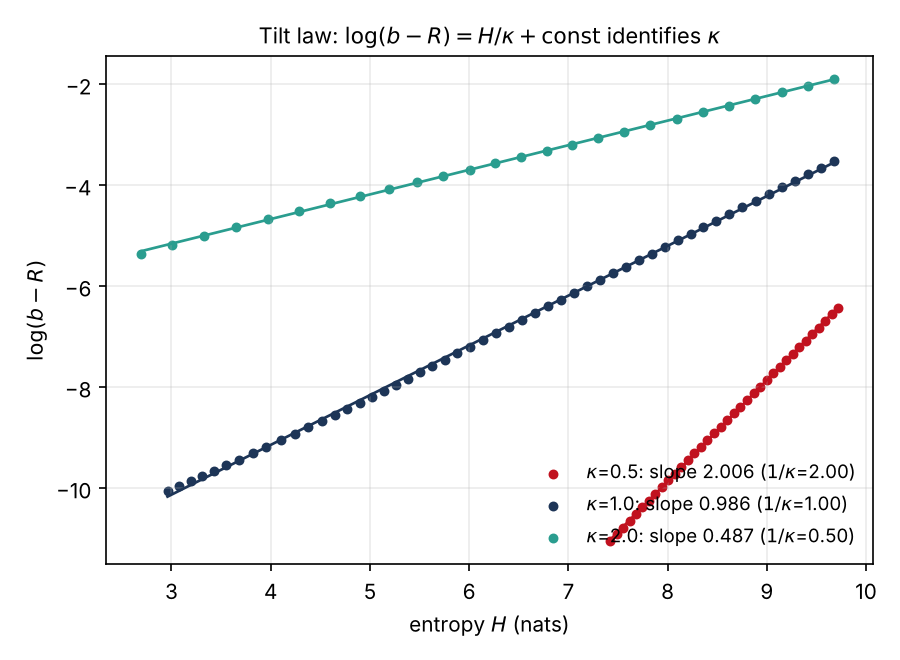
\includegraphics[width=0.62\linewidth]{fig3_tiltlaw.png}
\caption{The tilt law. For base-fitness crowding exponents $\kappa\in\{0.5,1,2\}$,
$\log(b-R)$ is linear in the entropy $H$ with slope $1/\kappa$. Fitted slopes are
$2.006,\,0.986,\,0.487$ against the predicted $2,\,1,\,0.5$ (within $2.6\%$). The
slope identifies $\kappa$ from a single entropy-reward trace.}
\label{fig:tiltlaw}
\end{figure}

\paragraph{What is ours, what is concurrent.}
The exponential form at $\kappa=1$ is due to Cui et al.; the identifiable
exponent $\kappa$ and its reading as near-optimal crowding are the contribution
here. The exact entropy-mass curve, the shifted-exponential as a finite-window
approximation with error bounds, and the proof that the true terminal law is not
exponential are concurrent work (Winner-Take-All, S4R2zYtFhs); we do not claim
them, and \eqref{eq:tiltlaw} is stated as a mesoscopic law, not a global one. Our
use of the tilt is to connect this entropy side to the pass@$k$ side through the
one identity of Theorem \ref{thm:tilt}.

\subsection{Entropy collapse and the bump}
\label{sec:entropy}

Along the tilt the entropy moves by the exact identity of Lemma \ref{lem:bump},
$\tfrac{\mathrm d}{\mathrm d\tau}H(\wt)=-\Cov_{\wt}(f,\log\wz)-\tau\Var_{\wt}(f)$:
with a uniform base $H$ is nonincreasing and collapses to $\log|\arg\max f|$, and
with a nonuniform base it rises first iff $\Cov_{\wz}(f,\log\wz)<0$.

The collapse to a single-strategy support is the strategy-level counterpart of
the winner-take-all concentration analyzed in concurrent work; the bump
condition names exactly when the transient rise seen in training occurs. We
state these at the \emph{strategy} level: token entropy need not track strategy
entropy, because a concentrating policy can still spread probability within the
surviving strategy. The accompanying package exhibits a case where strategy
entropy falls from $2.77$ to $2.14$ while token entropy rises from $6.85$ to
$7.27$, so any entropy-performance statement here is about strategies, not
tokens. This is the same family-versus-token distinction identified empirically
in concurrent work, and it is why Theorem \ref{thm:tiltlaw} is a strategy-level
law.

\paragraph{Verification.}
The entropy identity of Lemma \ref{lem:bump} holds to $2\times10^{-6}$ under a
uniform base, the predicted bump appears under a nonuniform base, and the tilt
law slopes match $1/\kappa$ within $2.6\%$ (Figure \ref{fig:tiltlaw}). All three
are regenerated and checked by the package.